\chapter{Réalisation}
\label{chap:Réalisation}


L’implémentation est la phase la plus importante après celle de la conception. Le choix
des outils de développement influence énormément sur le coût en temps de programmation, ainsi que sur la flexibilité du produit à réaliser. Cette phase consiste à transformer
le modèle conceptuel établi précédemment en des composants logiciels formant notre système. Dans ce chapitre, nous allons présenter d’une façon succincte les différents outils
dont on s’est servi tout au long de la réalisation de notre application.
\pagebreak
\section{Langages et technologies de développement utilisés}


\subsection{Modélisation : Langage UML}

\begin{figure}[H]
    \centering
    
\includegraphics[scale=0.15]{Logos/UML_logo.png}
    \caption{Logo UML}
\end{figure}

Pour concevoir notre système, nous avons choisi UML comme un
langage de modélisation, notre choix s’est basé sur les points forts de
ce langage comme la standardisation et les divers diagrammes qu’il
propose.En effet, Le langage UML (Unified Modeling Language, ou langage de modélisation unifié) a été pensé pour être un langage de modélisation visuelle commun, et riche sémantiquement et syntaxiquement. Il est destiné à l'architecture, la conception et la mise en œuvre de systèmes logiciels complexes par leur structure aussi bien que leur comportement. L'UML a des applications qui vont au-delà du développement logiciel, notamment pour les flux de processus dans l'industrie \cite{UML}.

\subsection{Couche présentation}

\subsubsection{HTML}

\begin{figure}[H]
    \centering
    
\includegraphics[scale=0.3]{Logos/html.png}
    \caption{Logo HTML}
\end{figure}

HTML est un langage de balisage conçu pour représenter
les pages web. C’est un langage permettant d’écrire de l’hypertexte, d’où son nom. HTML permet également de structurer sémantiquement et logiquement et de mettre en forme
le contenu des pages, d’inclure des ressources multimédias
dont des images, des formulaires de saisie et des programmes
informatiques.

\subsubsection{CSS}

\begin{figure}[H]
    \centering
    
\includegraphics[scale=0.3]{Logos/css.png}
    \caption{Logo CSS}
\end{figure}

CSS (pour Cascading Style Sheets en anglais), soit feuilles de style en cascade, est un langage de feuille de style utilisé pour décrire la présentation d'un document écrit en HTML ou XML (y compris les dialects XML que sont SVG, MathML, ou XHTML). CSS décrit la façon dont les éléments doivent être affichés à l'écran, sur papier, à l'oral ou sur d'autres médias.

\subsubsection{TypeScript}

\begin{figure}[H]
    \centering
    
\includegraphics[scale=0.05]{Logos/Typescript.png}
    \caption{Logo TypeScript}
\end{figure}

TypeScript est un langage de programmation libre et open-source développé par Microsoft qui a pour but d'améliorer et de sécuriser la production de code JavaScript. Il s'agit d'un sur-ensemble syntaxique strict de JavaScript.

TypeScript a une relation inhabituelle avec JavaScript. TypeScript offre toutes les fonctionnalités de JavaScript, avec une couche supplémentaire de fonctionnalités : le système de typage.

JavaScript fournit des primitives, comme string et number, mais aucune vérification n’est faite pour s’assurer que les assignations que vous faites sont correctes. TypeScript le fait.

Cela signifie que votre code JavaScript existant est également du code TypeScript. L’avantage principal de TypeScript est sa capacité à exposer les comportements imprévus dans votre code, diminuant les risques de bugs.\cite{Typescript}

\subsection{Couche traitement : 4D}

\begin{figure}[H]
    \centering
    
\includegraphics[scale=0.8]{Logos/Logo-4D.jpg}
    \caption{Logo 4D}
\end{figure}

Le langage 4D est un langage de programmation spécifique à la plateforme utilisé dans l’environnement de développement 4D pour créer des applications professionnelles et
des bases de données. Il est conçu pour simplifier le développement d’applications en fournissant des fonctionnalités
spécifiques à la gestion des données et des interfaces utilisateur.

\section{Librairies et frameworks utilisés}

\subsection{Couche présentation}

\subsubsection{React}


\begin{figure}[H]
    \centering
    
\includegraphics[scale=0.2]{Logos/react.png}
    \caption{Logo React}
\end{figure}

React est une bibliothèque JavaScript frontale open
source permettant de créer des interfaces utilisateur ou des
composants d’interface utilisateur. Il est maintenu par Facebook et une communauté de développeurs individuels et
d’entreprises. React peut être utilisé comme base dans le développement d’applications monopages ou mobiles.

\subsubsection{Tailwind}

\begin{figure}[H]
    \centering
    
\includegraphics[scale=0.5]{Logos/tailwind.png}
    \caption{Logo Tailwind}
\end{figure}

Tailwind CSS est un framework CSS open source. La fonctionnalité principale de cette bibliothèque est, contrairement à d'autres frameworks CSS comme Bootstrap, qu'elle ne procure pas une série de classes prédéfinies pour des éléments tels que des boutons ou des tables. À la place, Tailwind crée une liste de classes CSS « utilitaires » pouvant être utilisés pour ajouter un style à chaque élément en les mélangeant et en les agençant.

\subsubsection{Axios}

\begin{figure}[H]
    \centering
    
\includegraphics[scale=0.5]{Logos/axios.png}
    \caption{Logo Axios}
\end{figure}

Lors de la création d’une application Web, il est fréquent de vouloir utiliser et afficher les données provenant d’une API. Il existe plusieurs manières de le faire, à savoir :
   
- API Axios : Il s’agit d’un client HTTP basé sur les promesses pour le navigateur et Node.js. Il facilite l'envoi de requêtes HTTP asynchrones aux points de terminaison REST et la réalisation de plusieurs opérations. Il peut être utilisé en JavaScript simple ou avec une bibliothèque telle que React.

- API Fetch : Elle fournit une interface JavaScript pour l'accès et la manipulation des parties du pipeline HTTP, comme les requêtes et les réponses. Cela fournit aussi une méthode globale qui procure un moyen facile et logique de récupérer des ressources à travers le réseau de manière asynchrone.

Nous avons choisi de travailler avec Axios puisqu’il fournit une API facile à utiliser dans un package compact pour la plupart des besoins de communication http 

\section{Environnements et outils de développement utilisés}

\subsection{Visual Studio Code }

\begin{figure}[H]
    \centering
    
\includegraphics[scale=0.25]{Logos/VS.jpg}
    \caption{Logo Visual Studio Code }
\end{figure}

Visual Studio Code est éditeur de texte open source, gratuit et multiplateforme (Windows, Mac et Linux), développé
par Microsoft. Principalement conçu pour le développement
d’application avec JavaScript, Type script et Node.js, l’éditeur peut s’adapter à d’autres types de langages grâce à un
Système d’extension bien fourni. \cite{VS}

\subsection{4D Client}

\begin{figure}[H]
    \centering
    
\includegraphics[scale=0.5]{Logos/4dClient.PNG}
    \caption{Logo  4D client}
\end{figure}
4D vous permet de construire des applications clientserveur personnalisées qui sont homogènes, multiplateformes
et avec une option de mise à jour automatique. Les applications client et serveur sont configurées dans la page
Client/Serveur de la boîte de dialogue Construire une application.

\subsection{4D Serveur}


\begin{figure}[H]
    \centering
    
\includegraphics[scale=1.5]{Logos/4dServeyr.PNG}
    \caption{Logo 4D Serveur}
\end{figure}

4D Server est un composant logiciel de la plateforme de
développement 4D qui permet le déploiement et la gestion d’applications client-serveur. Il offre un environnement robuste et évolutif pour héberger des applications 4D, permettant à plusieurs utilisateurs d’y accéder et d’interagir avec
l’application simultanément. 4D Server agit comme un hub centralisé, gérant le stockage
des données, le traitement et la communication entre le serveur et les applications clientes
connectées. Il prend en charge des fonctionnalités telles que l’accès simultané aux données partagées, la gestion des transactions, les contrôles de sécurité et la collaboration
multi-utilisateur.

\subsection{Postman}

\begin{figure}[H]
    \centering
    
\includegraphics[scale=0.5]{Logos/postman.png}
    \caption{Logo  Postman}
\end{figure}

Postman est la solution la plus populaire pour tester / appeler une API Web. Postman offre un environnement graphique complet qui permet de gérer toutes les interactions avec les API Web. Les requêtes construites et exécutées sont stockées dans une histoire facilitant ainsi leur ré-exécution. \cite{Postman}

\subsection{GitLab}

\begin{figure}[H]
    \centering
    
\includegraphics[scale=0.1]{Logos/gitlab.jpg}
    \caption{Logo GitLab}
\end{figure}

GitLab est une plateforme DevOps complète proposée
sous la forme d’une application unique. Elle révolutionne le
développement, la sécurité, l’exploitation et la collaboration
entre les équipes. Créez, testez et déployez des logiciels plus
rapidement en n’utilisant qu’une seule solution. \cite{GitLab}

\subsection{Git}

\begin{figure}[H]
    \centering
    
\includegraphics[scale=0.5]{Logos/git.png}
    \caption{Logo Git}
\end{figure}

Git est un logiciel qui permet d’effectuer un contrôle de
 version. Ce grand projet nécessitait un 
 logiciel pour suivre toutes les modifications apportées à une base de code afin de suivre des choses comme : Qui a édité un certain fichier, ce qu'on a changé et comment revenir au code d'origine si nécessaire.

 \subsection{StarUML}

 \begin{figure}[H]
    \centering
    
\includegraphics[scale=0.4]{Logos/starUml.png}
    \caption{Logo  StarUML}
\end{figure}
 
 StarUML est un logiciel de modélisation UML (Unified Modeling Language) open source
qui peut remplacer dans bien des situations des logiciels commerciaux et coûteux
comme Rational Rose1 ou Together2
. Étant simple d’utilisation, nécessitant peu de
ressources système, supportant UML 2, ce logiciel constitue une excellente option pour
une familiarisation à la modélisation. Cependant, seule une version Windows est disponible. \cite{StarUml}

\section{base de données }

La plateforme 4D intègre un système de gestion de base de données (SGBD)qui permet le stockage, la gestion et la manipulation des données. nous  utilisons le composant structure pour créer graphiquement les tables de notre base de données, En suivant  un ensemble de règles de 4D .

Nous  séparons la catégorie des cours dans une table distincte. Cela permet de gérer les gèrer  de manière centralisée et de faciliter leur mise à jour. Si la catégorie des cours change, il suffit de modifier la table des catégories et les modifications seront automatiquement répercutées sur tous les cours qui y sont associés.

De même, nous séparons  la table des rôles pour prendre en compte l'ajout de nouveaux rôles. Cela permet de gérer les rôles de manière indépendante et de faciliter leur gestion. Si un nouveau rôle est ajouté, il suffit de créer une nouvelle entrée dans la table des rôles et de lui associer les permissions nécessaires.

Enfin,  également la table " administrateur" pour faciliter la gestion des privilèges et des rôles. Cela permet de gérer les administrateurs de manière indépendante et de leur attribuer des permissions spécifiques. De plus,on séprons cette table nous garantissons que ses données ne peut pas etre accessible par un autre utilisateur. la figure suivante représente notre base de données :


\begin{figure}[H]
    \centering
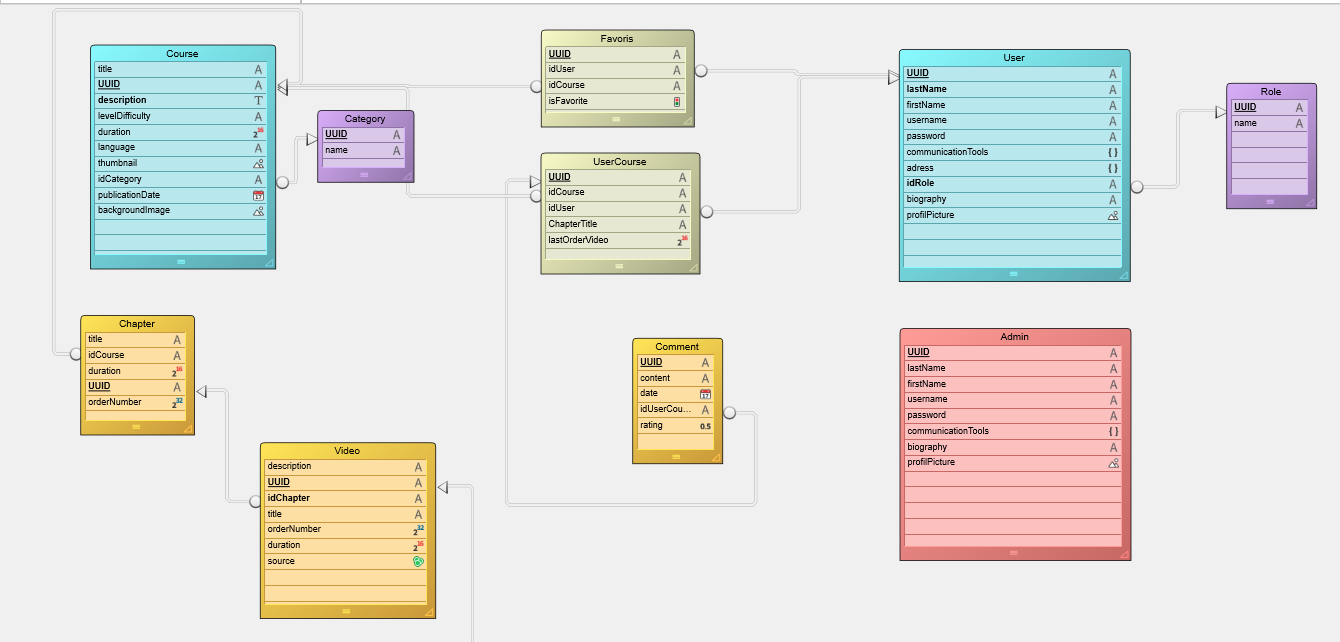
\includegraphics[width=19cm]{Figures/database.PNG}

    \caption{création de la base de données en 4D}
    \label{fig:4dmonde1}
\end{figure}

La gestion des relations entre les tables est un peu différente dans le SGBD 4D ,elle ne se fait pas seulement a travers les clès mais aussi via la création des liens avec des règles sont spécifique pour 4D. D'ailleurs, on peut seulement utiliser les liens N vers 1.

Lorsqu'on  trace un lien entre deux tables, la table contenant le champ clé primaire de la relation est appelée la Table 1 et la table contenant le champ clé d’appel de la relation est appelée la Table N. Ces tables sont appelées table 1 et table N car un enregistrement de la table 1 est relié à N enregistrements de la table N et inversement. Ce type de relation est appelé une relation de N vers 1.

Les liens 1 vers 1 ne sont pas utilisés car les tables qui sont liées par ce type de lien peuvent être combinées dans une table unique.

Pour manipuler les relations plusieurs-à-plusieurs nous utilisons ce qu'on appelle "Atribut Alias".En effet, Ils apportent plus de lisibilité et de simplicité dans le code et dans les recherches en permettant de s'appuyer sur des concepts métier plutôt que sur des détails d'implémentation.

Considérant le modèle suivant :

\begin{figure}[H]
    \centering
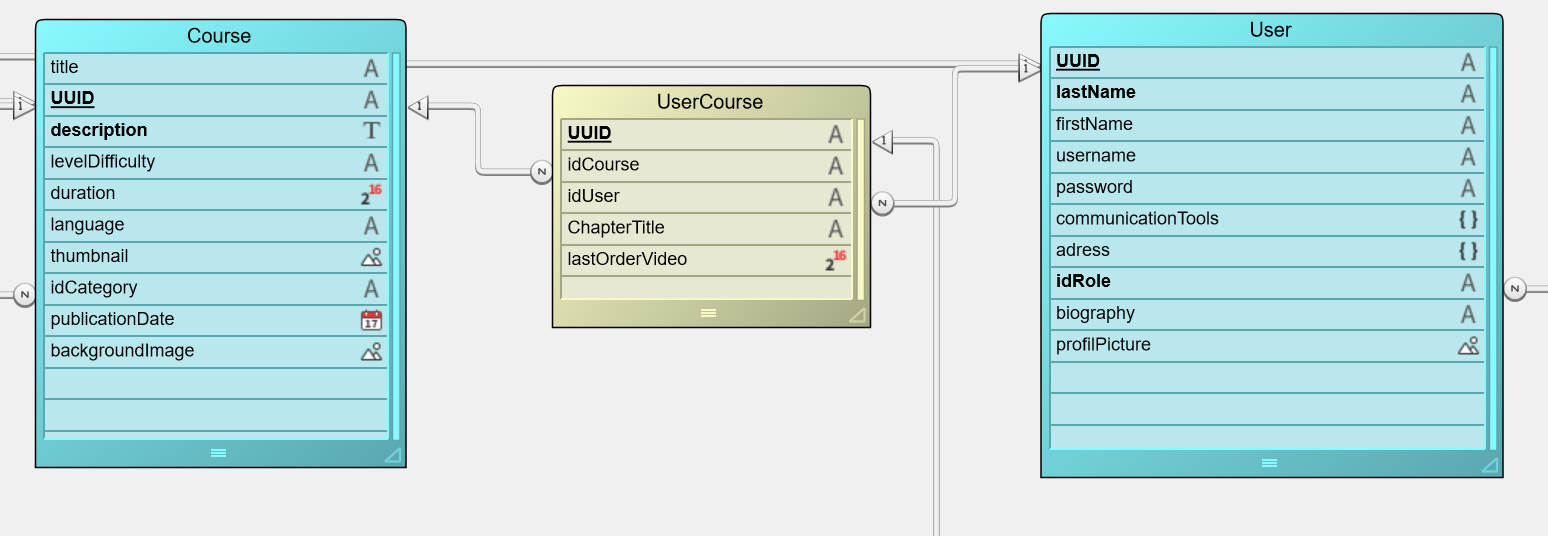
\includegraphics[width=19cm]{Figures/exemple.PNG}
    \caption{exemple de relation N vers N}
\end{figure}

Dans la dataclasse Course, l'attribut alias "client" renvoie tous les user d'une formation.

\begin{figure}[H]
    \centering
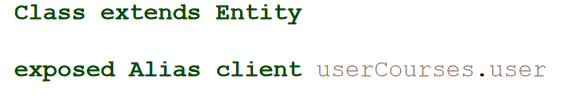
\includegraphics[width=10cm]{Figures/alias.PNG}
    \caption{Attribut Alias}
\end{figure}

\section{Sécurité}

\subsection{Implémentation des sessions}
Lorsque les sessions sont activées, des mécanismes automatiques sont mis en œuvre, basés sur un cookie privé défini par 4D lui-même : « 4DSID\_AppName », où AppName est le nom du projet d'application. Ce cookie fait référence à la session Web en cours pour l'application. 

Le nom du cookie peut être obtenu à l'aide de la propriété \texttt{.sessionCookieName}.



\begin{itemize}[label=$\checkmark$]
    \item Dans chaque requête du client web, le serveur Web vérifie la présence et la valeur du cookie privé "4DSID\_AppName".
    \item Si le cookie a une valeur, 4D recherche la session qui a créé ce cookie parmi les sessions existantes ; si cette session est trouvée, elle est réutilisée pour l'appel.
    \item Si la demande du client ne correspond pas à une session déjà ouverte :
    \begin{itemize}[label=$\bullet$]
        \item Une nouvelle session avec un cookie privé "4DSID\_AppName" est créée sur le serveur web.
        \item Un nouvel objet Session Invité est créé et est dédié à la session web évolutive.
    \end{itemize}
\end{itemize}

L'objet Session courant est alors accessible via la commande Session dans le code de n'importe quel processus Web.


\begin{figure}[H]
    \centering
    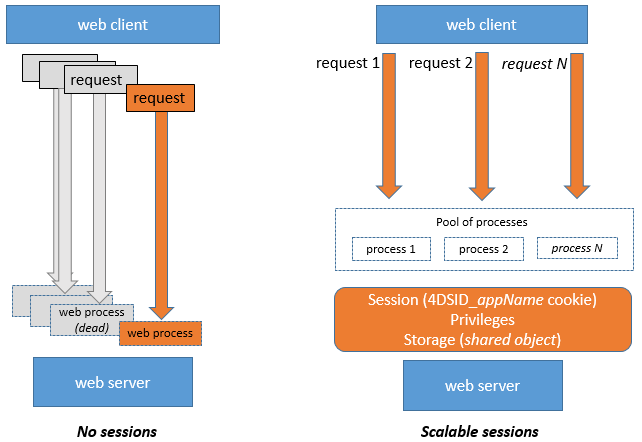
\includegraphics[width=19cm]{Figures/session.png}
    \caption{Schéma des sessions extensibles}
\end{figure}

\subsection{Roles et privilèges }

L'architecture de sécurité ORDA est basée sur les concepts de privilèges, d'actions d'autorisation (lecture, création, etc.) et de ressources.

Lorsque les utilisateurs sont connectés, leur session est automatiquement chargée avec les privilèges associés. Les privilèges sont attribués à la session à l'aide de la session.setPrivileges()fonction.

En roles.json : Chaque demande d'utilisateur envoyée au cours de la session est évaluée par rapport aux privilèges définis dans le fichier du projet .

Si un utilisateur tente d'exécuter une action et ne dispose pas des droits d'accès appropriés, une erreur de privilège est générée ou, en cas d'autorisation de lecture manquante sur les attributs, ceux-ci ne sont pas envoyés.


\begin{figure}[H]
    \centering
    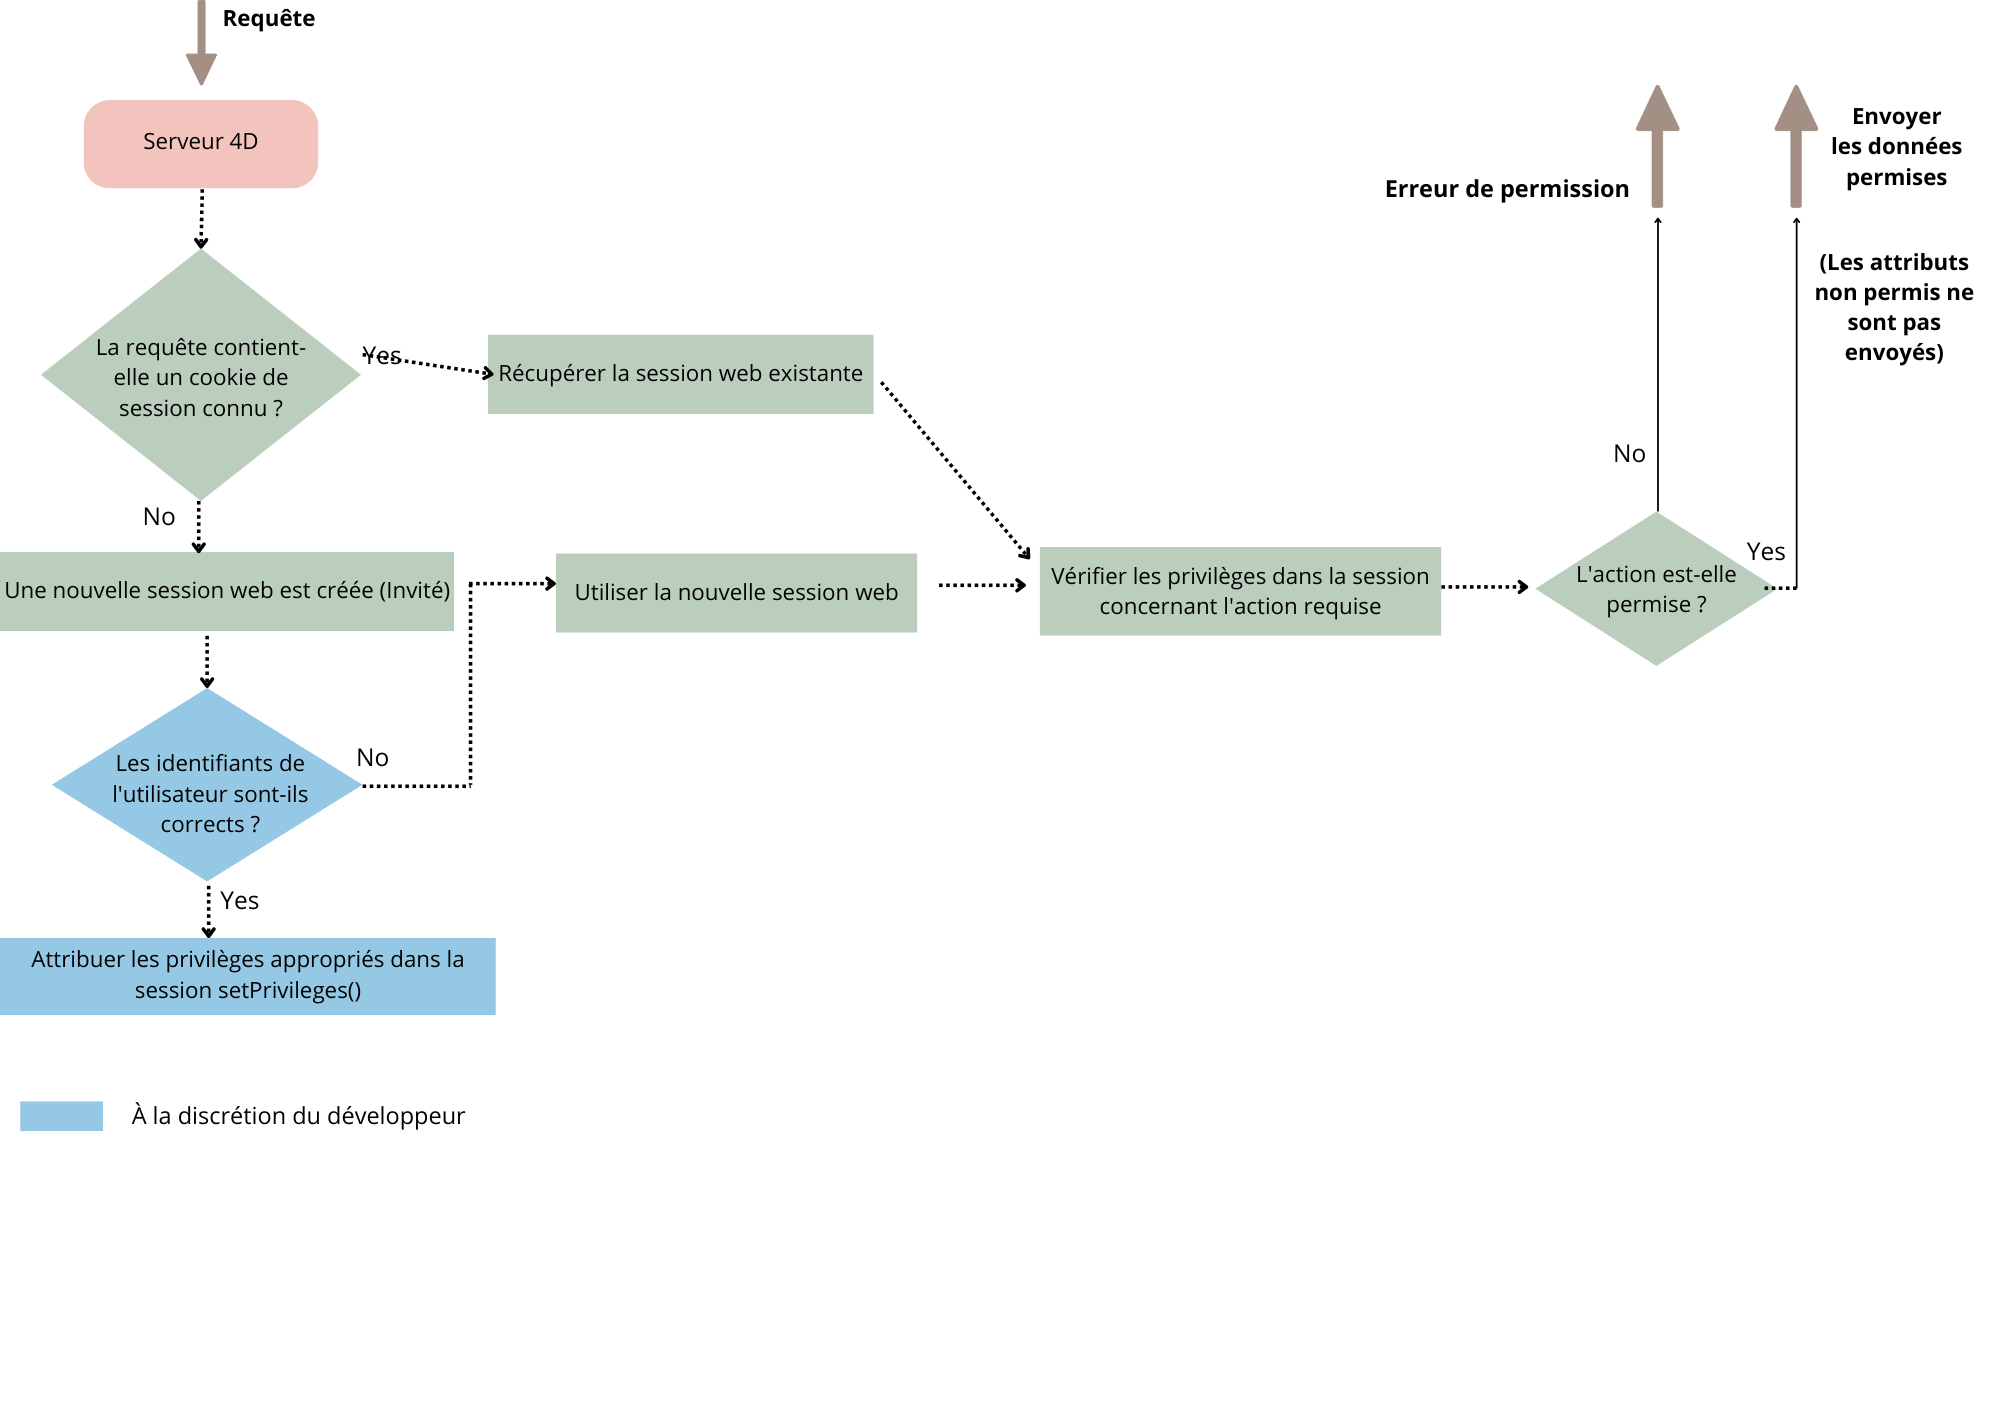
\includegraphics[width=19cm]{Figures/privilege.png}
    \caption{Schéma des privilèges en 4D}
\end{figure}

\section{Travail Réalisé}

La réalisation de l’application constitue une étape cruciale du processus de développement, où l’ensemble des concepts et solutions préalablement étudiés sont intégrés et mis en œuvre. Ce chapitre se focalise sur les deux principaux espaces implémentés : l’Espace Apprenant et l’Espace Administrateur.

\subsection{Authentification}

Pour accéder à leur espace personnel, les utilisateurs doivent s'authentifier en utilisant leur adresse électronique ou nom d'utilisateur et un mot de passe. Cette étape d'authentification permet de sécuriser l'accès à la plateforme et de diriger les utilisateurs vers leur interface spécifique selon leur rôle : apprenant ou administrateur.


\begin{figure}[H]
    \centering
    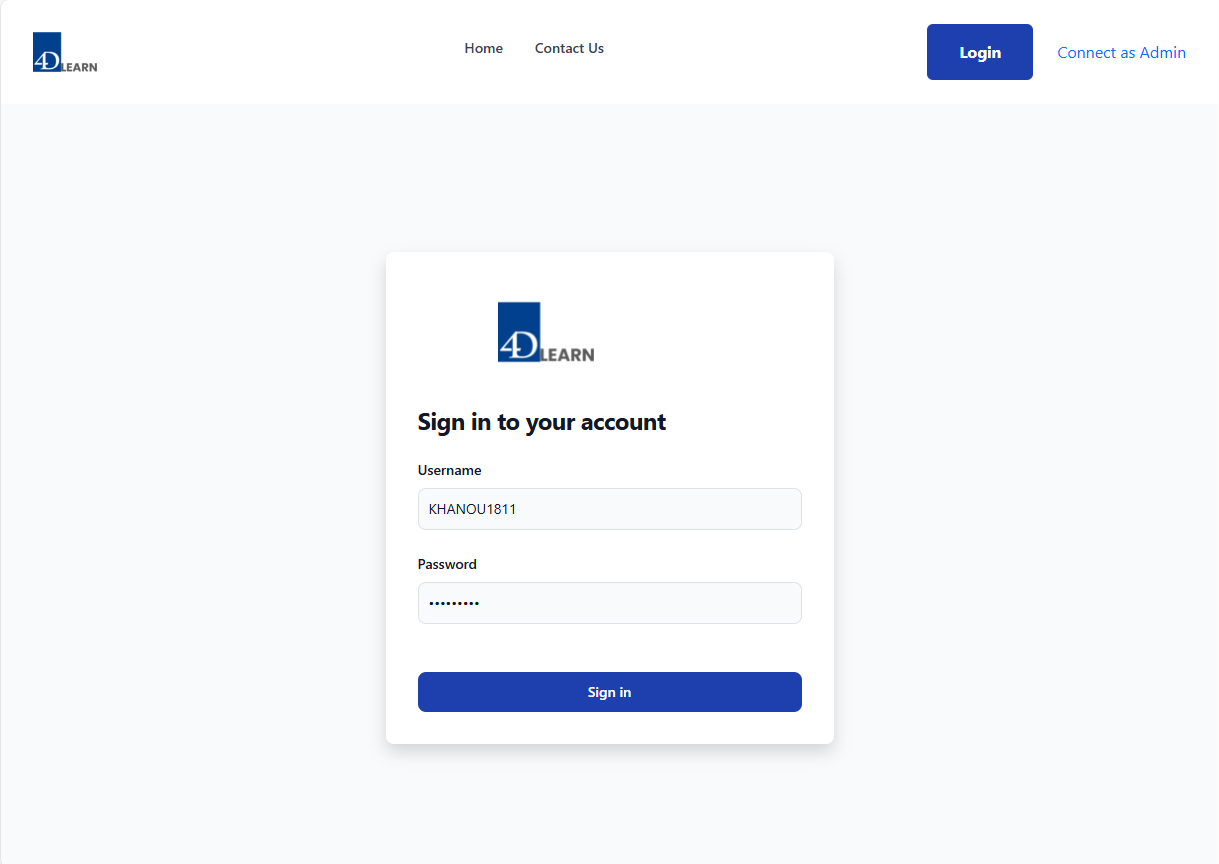
\includegraphics[width=19cm]{Figures/authntification.png}
    \caption{La page d'authentification}
\end{figure}

\subsection{Espace Apprenant }

L'Espace Apprenant est conçu pour offrir aux apprenants une interface intuitive et fonctionnelle, leur permettant d'accéder aux différentes ressources et fonctionnalités de la plateforme.

\subsubsection{Liste des formations}

Cette page présente une liste des formations disponibles. Les utilisateurs peuvent rechercher et filtrer les formations en fonction de divers critères tels que la catégorie, la langue, le niveau de difficulté et l’ordre.


\begin{figure}[H]
    \centering
    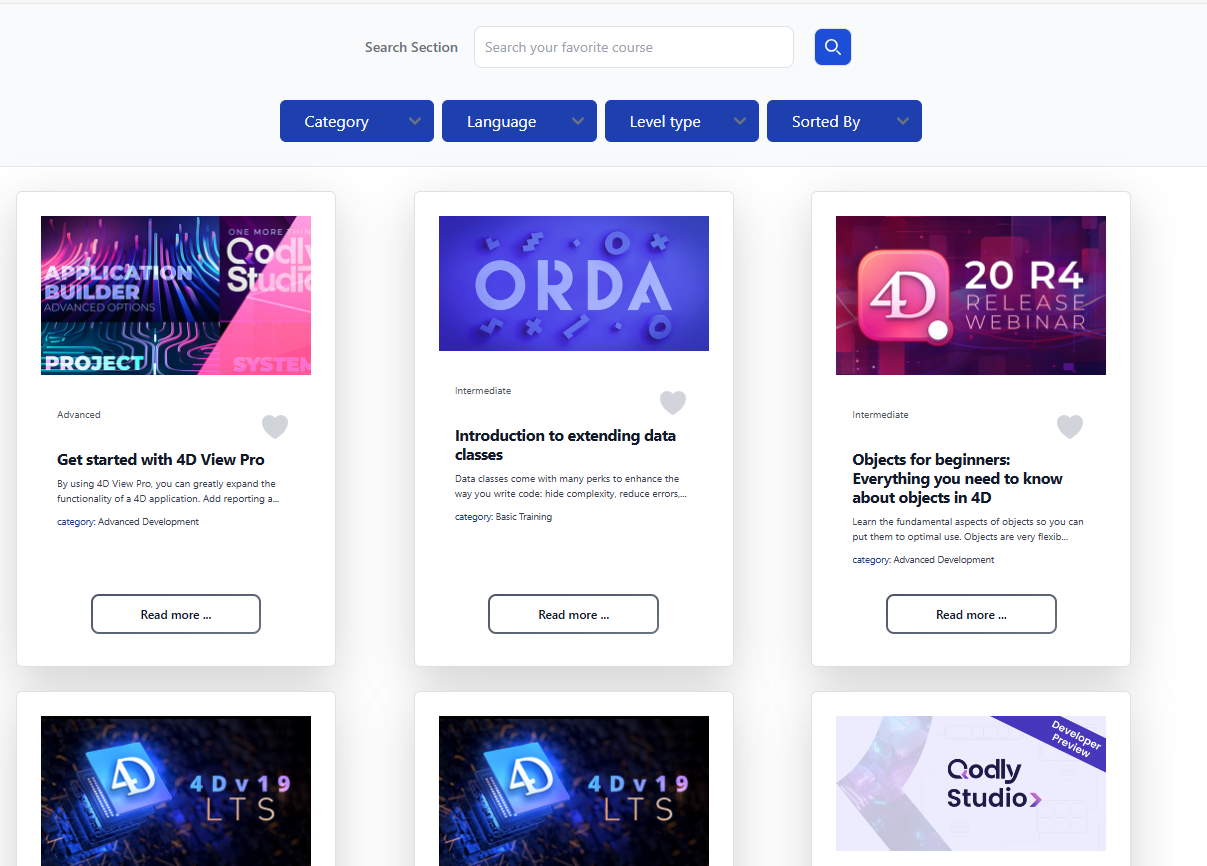
\includegraphics[width=19cm]{Figures/formations.png}
    \caption{Liste des formations}
\end{figure}

\subsubsection{Détails de la formation}

Cette page fournit des informations détaillées sur une formation spécifique, y compris le contenu du cours, infos générales et les évaluations.

\begin{figure}[H]
    \centering
    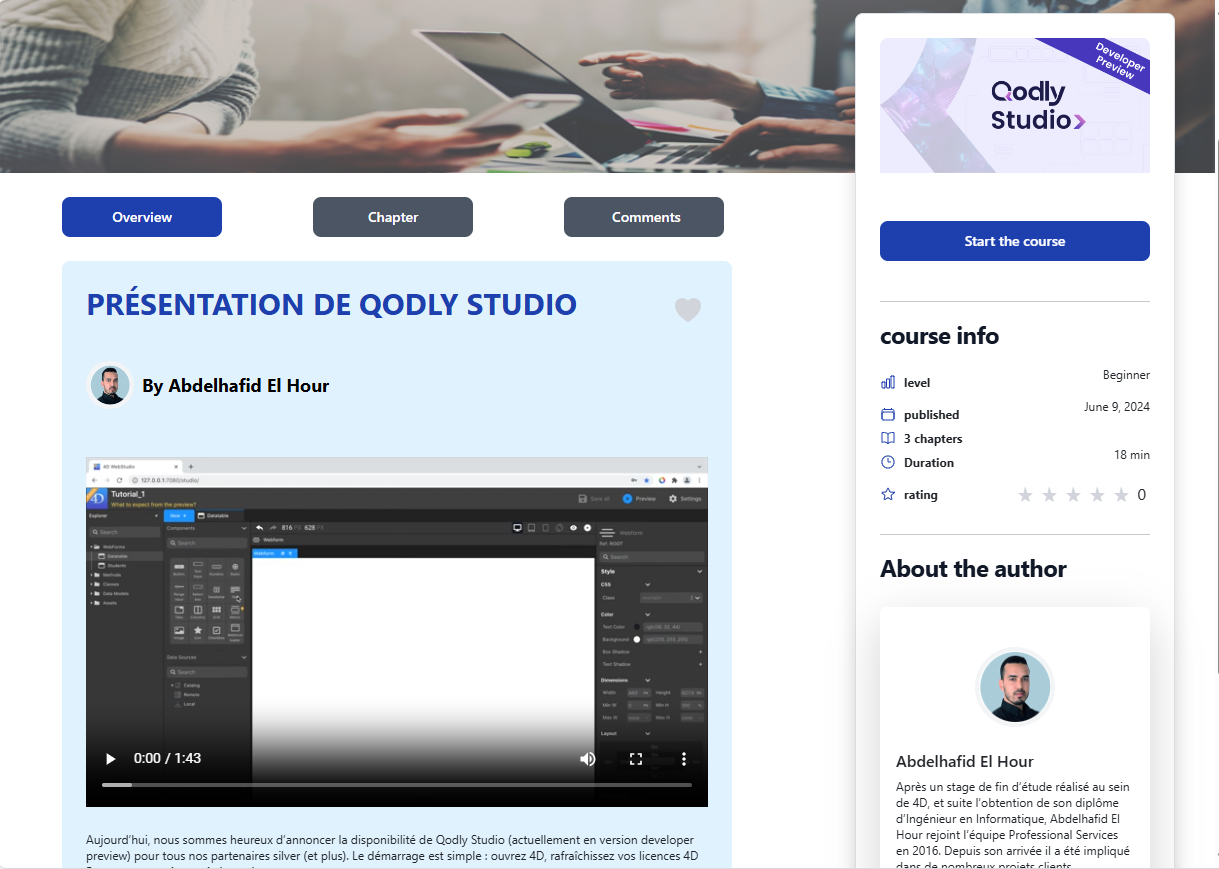
\includegraphics[width=19cm]{Figures/formation.png}
    \caption{Détails d'une formation}
\end{figure}

\subsubsection{Regarder formation}

Cette page permet aux apprenants de suivre une formation qu'ils ont choisie. Elle comprend les chapitres, les vidéos et les documents à télécharger.

\begin{figure}[H]
    \centering
    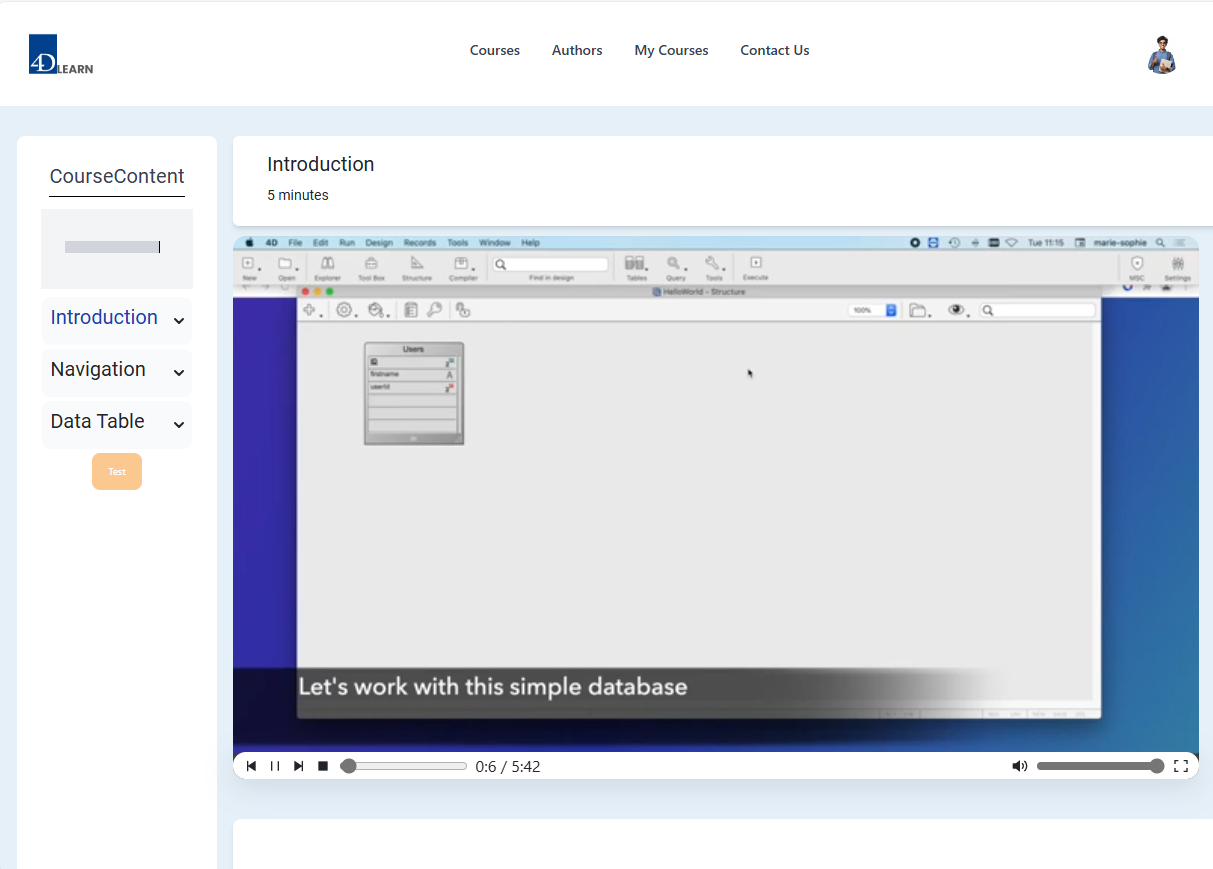
\includegraphics[width=19cm]{Figures/video.png}
    \caption{regarder formation}
\end{figure}

\subsubsection{Liste des formateurs}

Cette page offre une vue d'ensemble du profil de l'apprenant, incluant ses informations personnelles et ses préférences.

\begin{figure}[H]
    \centering
    
\includegraphics[width=19cm]{Figures/authors.png}
    \caption{la liste des formateurs}
\end{figure}

\subsubsection{Historique}

Cette page affiche l'historique des formations suivies par l'apprenant, y compris les formations terminées et en cours.

\begin{figure}[H]
    \centering
    
\includegraphics[width=19cm]{Figures/historique.png}
    \caption{ Page d'historique}
\end{figure}

\subsubsection{Favoris}

Cette page permet aux apprenants de sauvegarder leurs formations préférées pour un accès rapide ultérieur.

\begin{figure}[H]
    \centering
    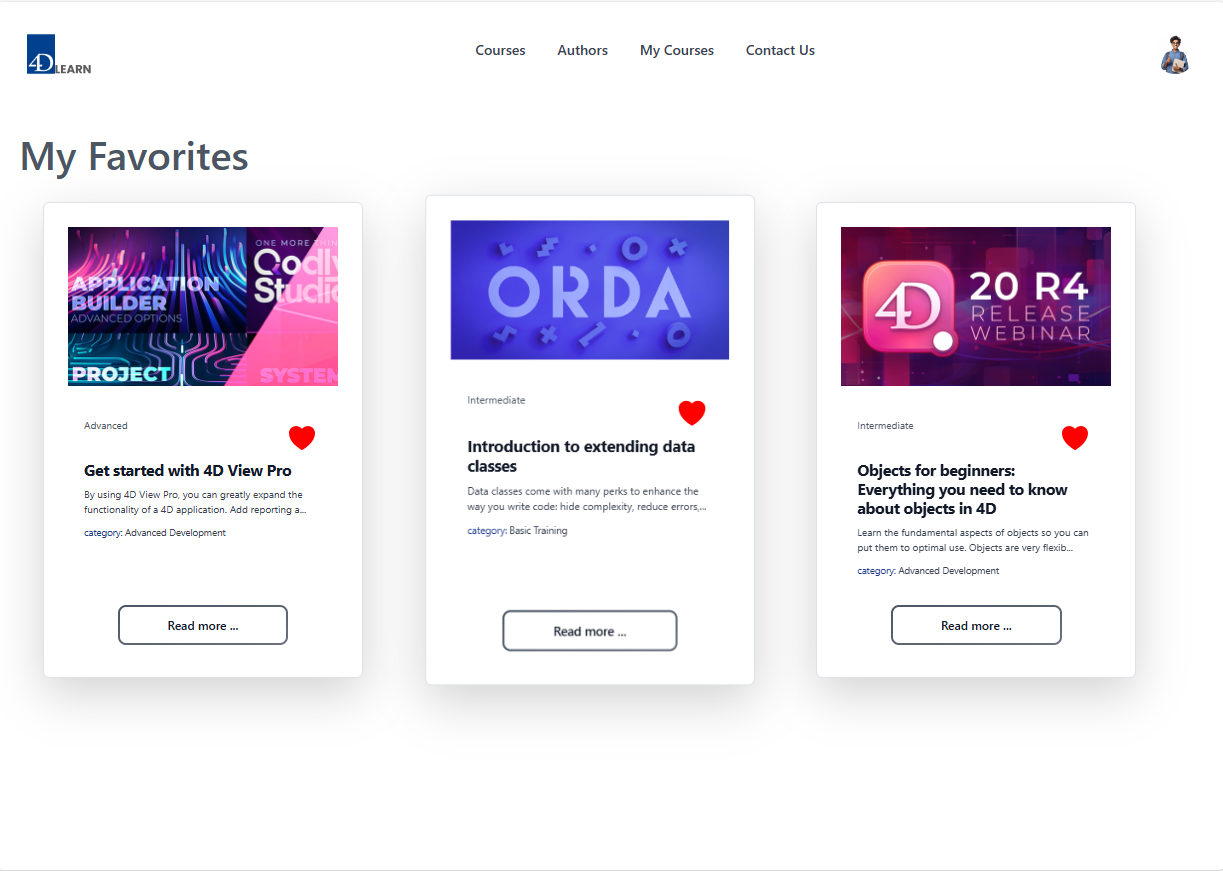
\includegraphics[width=19cm]{Figures/favoris.png}
    \caption{ Page de favoris}
\end{figure}

\subsubsection{Page de profil}
Cette page offre une vue d'ensemble du profil de l'apprenant, incluant ses informations personnelles.

\begin{figure}[H]
    \centering
    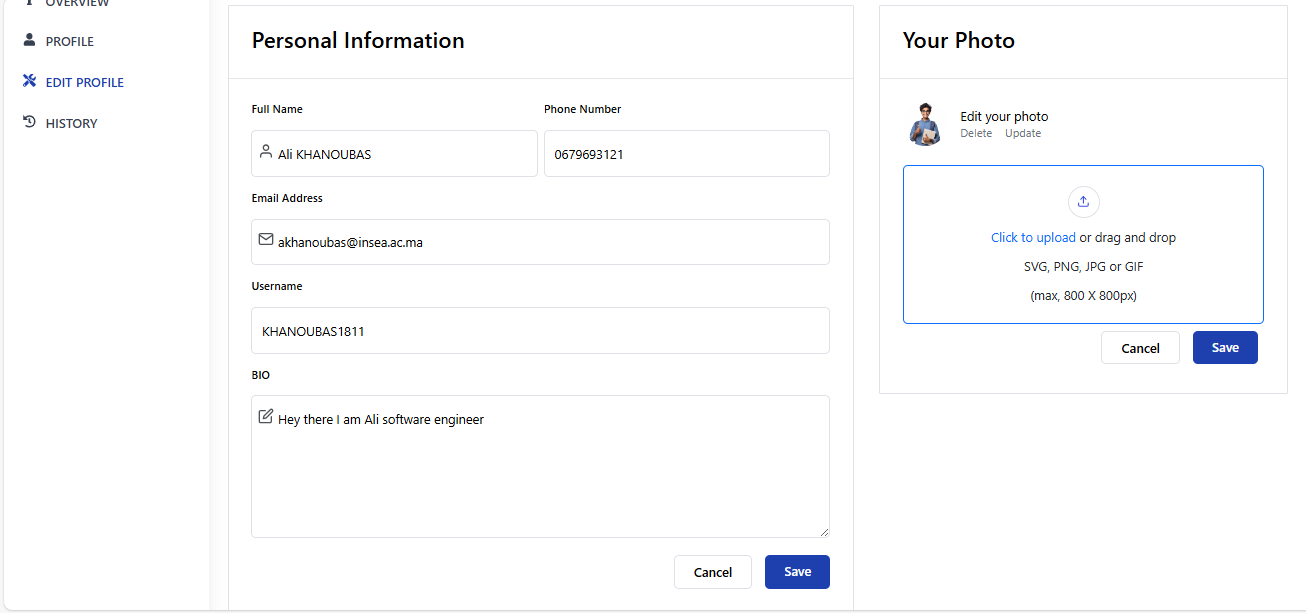
\includegraphics[width=19cm]{Figures/profil.png}
    \caption{ Page de profil}
\end{figure}


\subsubsection{Page de profile d’un formateur}

Cette page offre une vue détaillée du profil d'un auteur, incluant ses informations personnelles, ses qualifications, et les formations qu'il propose sur la plateforme.

\begin{figure}[H]
    \centering
    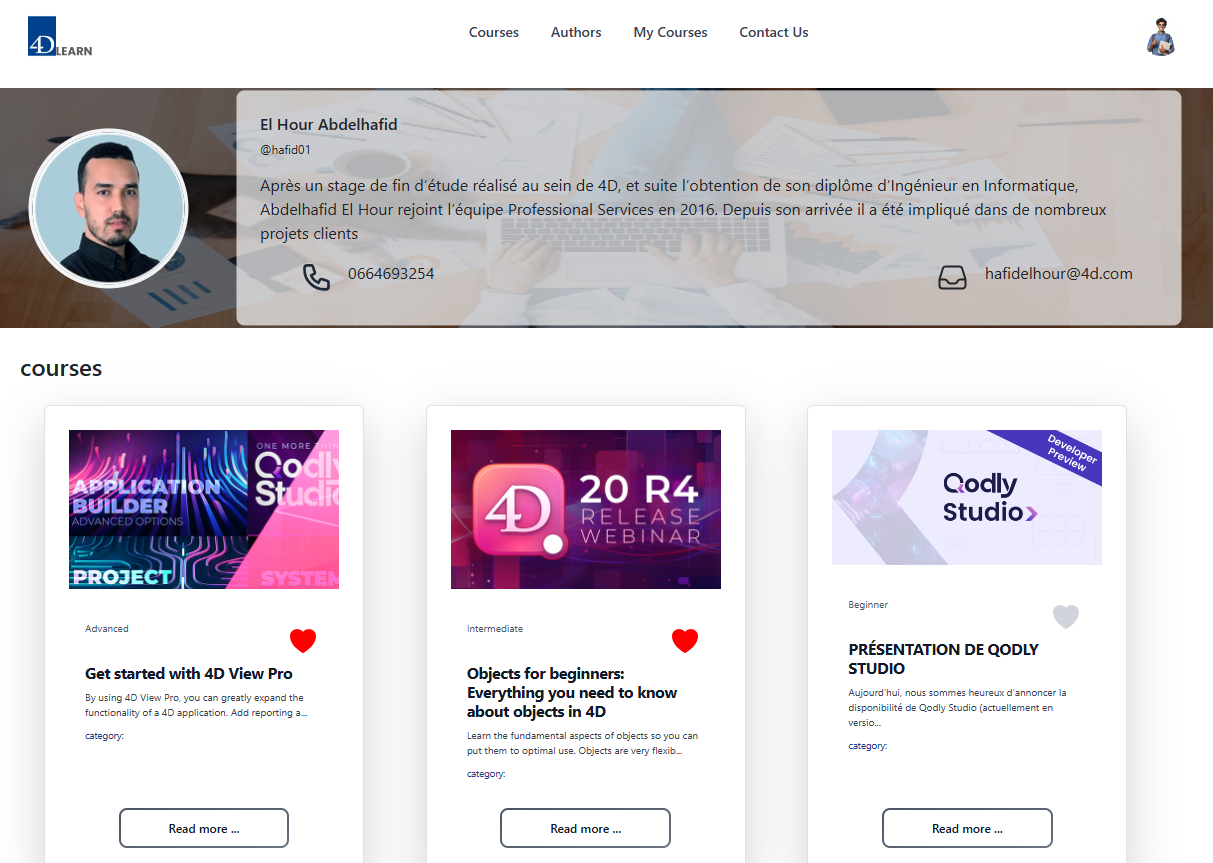
\includegraphics[width=19cm]{Figures/detailsAuthor.png}
    \caption{Page de profil d’un formateur}
\end{figure}

\subsection{Espace Administrateur}

L'Espace Administrateur est conçu pour permettre aux administrateurs de gérer la plateforme, les utilisateurs et les contenus de manière efficace.

\subsubsection{Tableau de bord}

Cette page fournit une vue d'ensemble des statistiques de la plateforme, y compris le nombre de formations, d'apprenants, d'auteurs, et autres indicateurs clés de performance.

\begin{figure}[H]
    \centering
    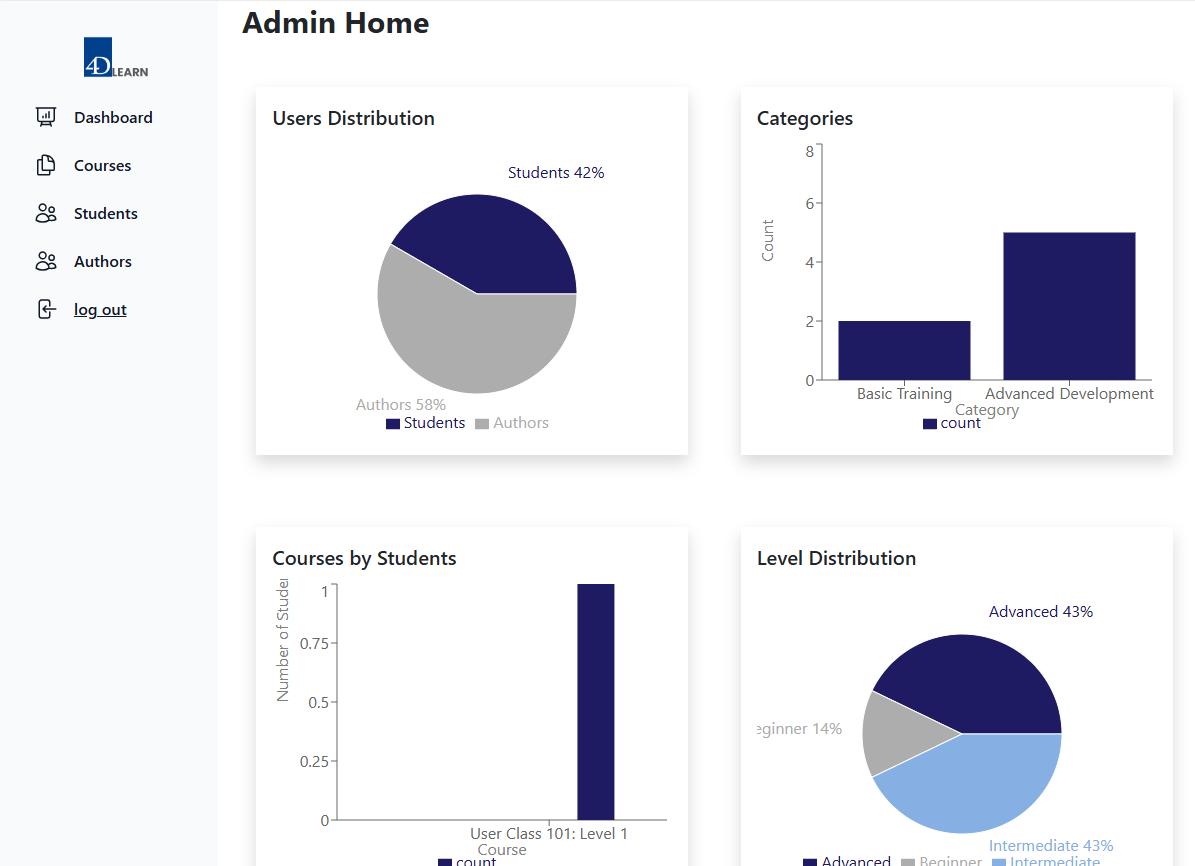
\includegraphics[width=19cm]{Figures/dashboard.png}
    \caption{ Page de tableau de bord}
\end{figure}

\subsubsection{Liste des formations et ajout formation}

Cette page permet aux administrateurs de visualiser toutes les formations disponibles et d'ajouter de nouvelles formations.

\begin{figure}[H]
    \centering
    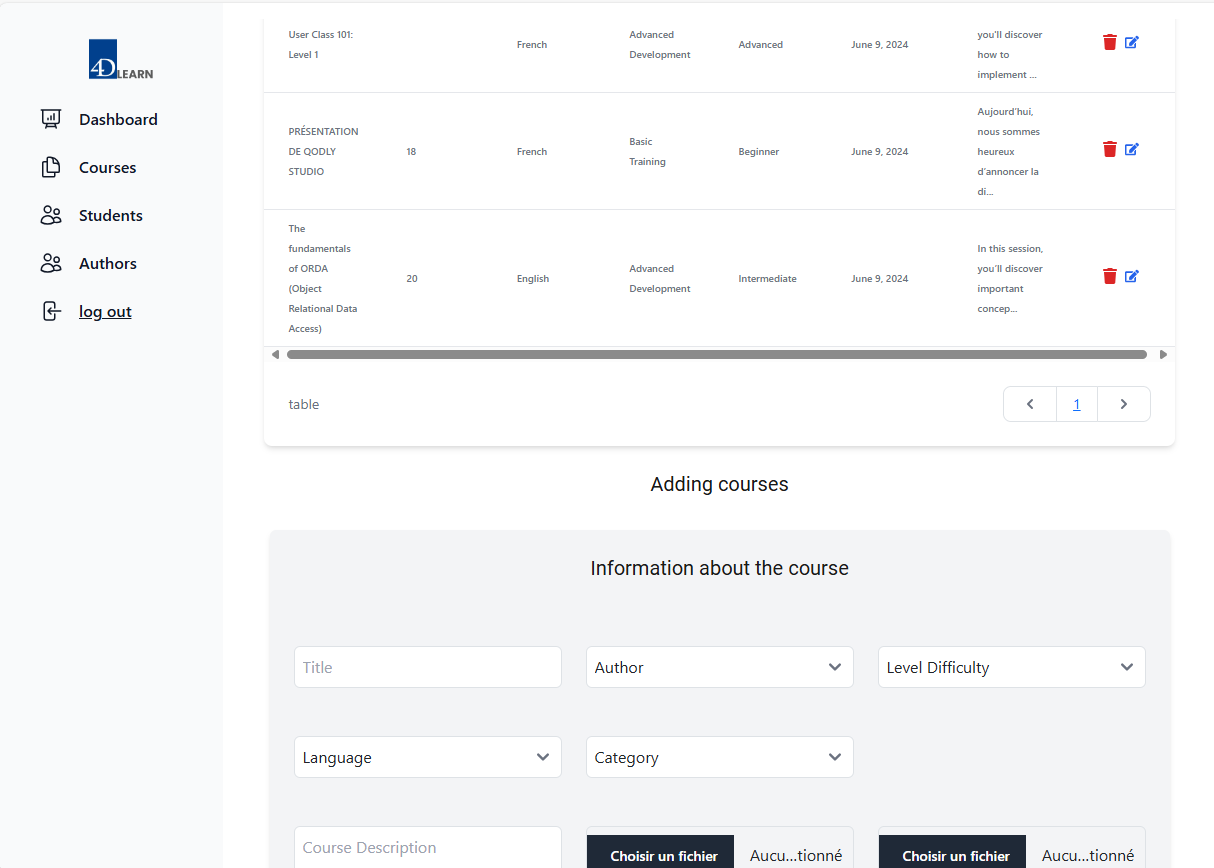
\includegraphics[width=19cm]{Figures/addCourse.png}
    \caption{ Page de Liste des formations + ajout formation}
\end{figure}

\subsubsection{Liste des formateurs et ajout formateur }

Cette page présente la liste des formateurs et permet l'ajout de nouveaux formateurs.

\begin{figure}[H]
    \centering
    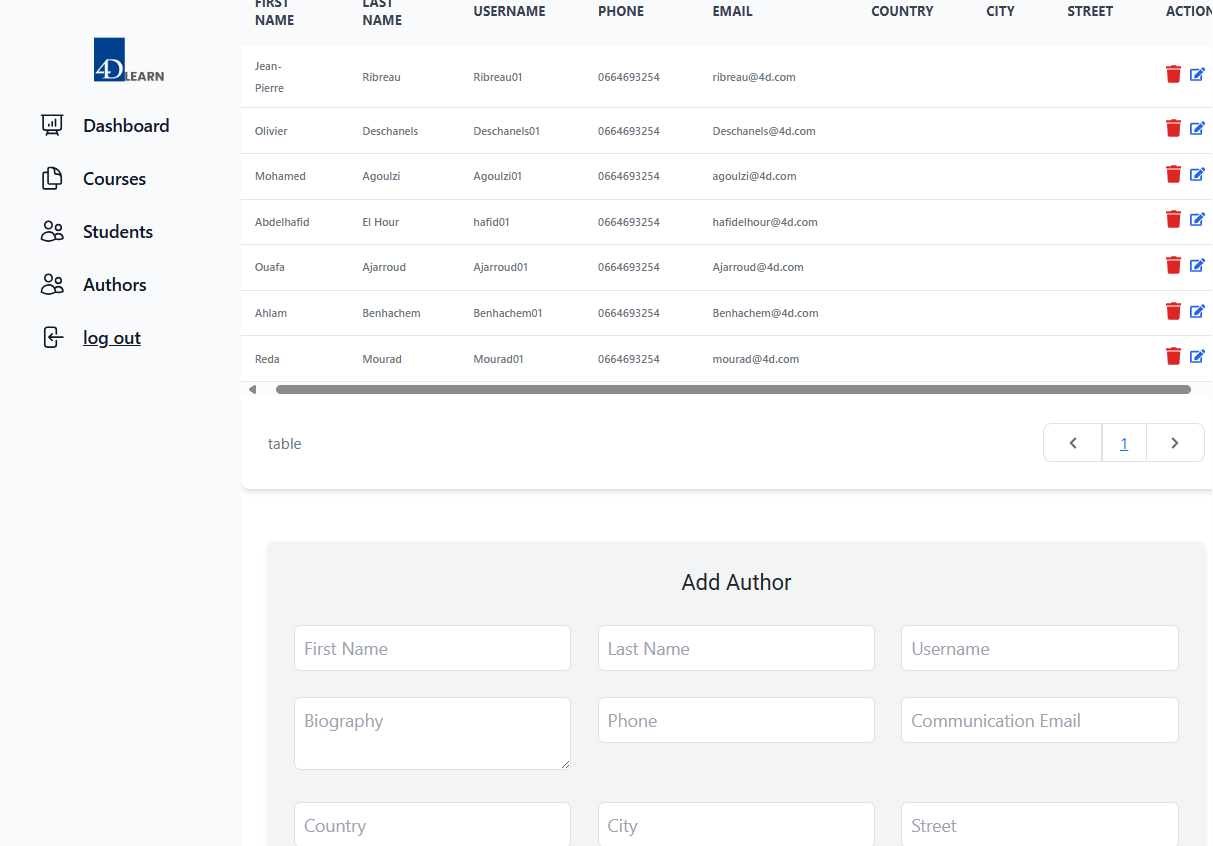
\includegraphics[width=19cm]{Figures/addAuthor.png}
    \caption{ Page de liste des formateurs et ajout formateur }
\end{figure}

\subsubsection{Liste des apprenants et ajout apprenant}

Cette page affiche la liste des apprenants inscrits sur la plateforme et permet l'ajout de nouveaux apprenants.

\begin{figure}[H]
    \centering
    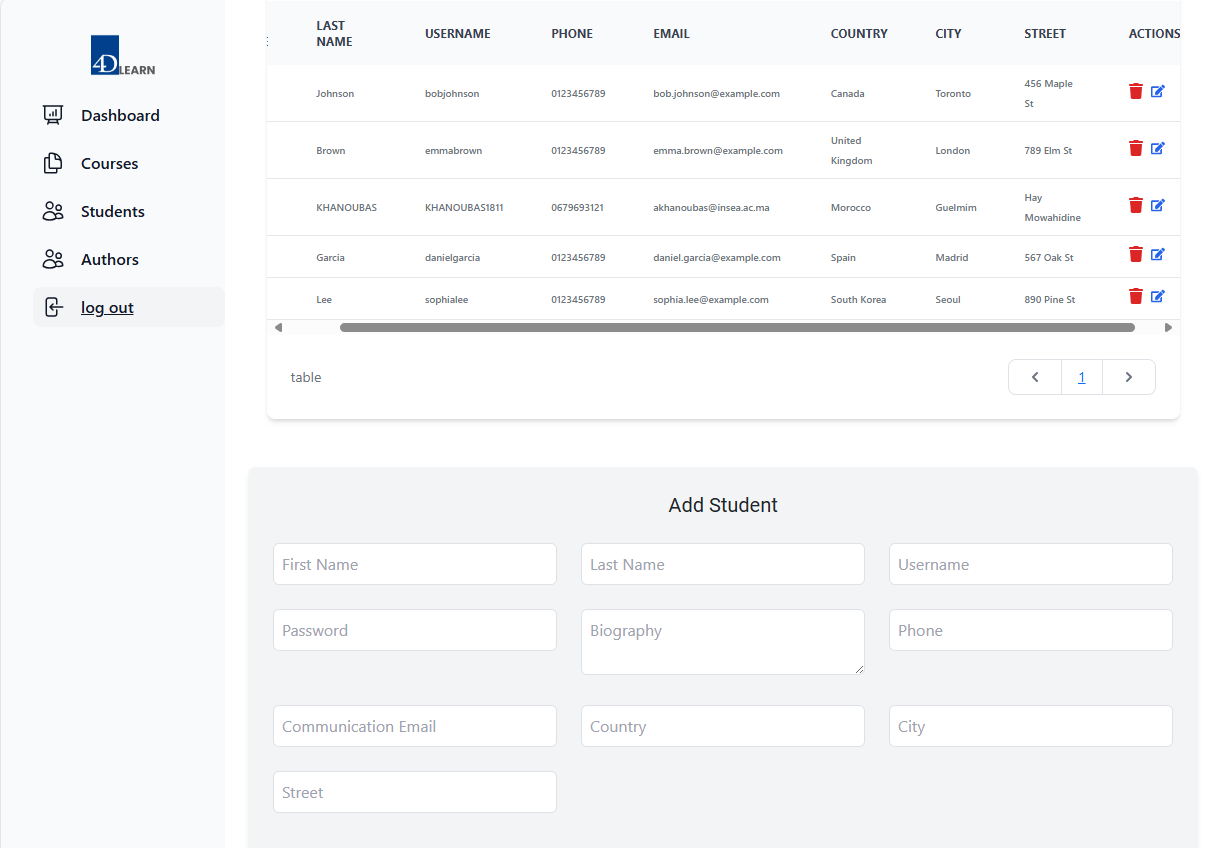
\includegraphics[width=19cm]{Figures/addStudent.png}
    \caption{ Page de liste des apprenants et ajout apprenant}
\end{figure}

\section{Validation des exigences}

\subsection{Exigences Fonctionnelles}
La validation des exigences est une étape cruciale pour s'assurer que toutes les fonctionnalités et les besoins du système sont correctement mis en œuvre. Voici les exigences fonctionnelles q'on a pu intégré dans notre plateforme:

\subsection{Authentification}

Pour valider l'exigence d'authentification, nous avons mis en place un système de connexion où les utilisateurs doivent saisir leur identifiant (email ou nom d'utilisateur) et leur mot de passe. Nous avons testé différentes combinaisons d'identifiants et de mots de passe pour vérifier que seuls les utilisateurs enregistrés peuvent accéder aux services.


\subsection{Gestion des Abonnements}

L'exigence de gestion des abonnements n'a pas encore été totalement intégrée, notamment en ce qui concerne le paiement. Actuellement, les utilisateurs peuvent s'inscrire aux formations sans payer. La validation de cette exigence a été faite en vérifiant que les utilisateurs peuvent s'inscrire à une formation après s'être authentifiés.


\subsection{Gestion des Formations pour les Apprenants}

Pour chaque sous-fonctionnalité de la gestion des formations, nous avons effectué des tests utilisateurs :
\begin{itemize}
    \item[$\bullet$] Inscription à une formation : Les utilisateurs ont pu s'inscrire à une formation après avoir authentifié. 
    \item[$\bullet$] Consultation d'une formation : Les utilisateurs inscrits ont pu accéder aux détails des formations.
    \item[$\bullet$] Évaluation d'une formation : Les utilisateurs ont pu laisser des évaluations après avoir suivi une formation.
    \item[$\bullet$] Recherche de formations : Les utilisateurs ont pu rechercher et trouver des formations spécifiques sur la plateforme.
    \item[$\bullet$] Consultation du profil d'un formateur : Les utilisateurs ont pu accéder aux profils des formateurs et consulter leurs informations.
\end{itemize}


\subsection{Gestion des Profils Apprenants}

Les utilisateurs ont pu modifier leurs informations personnelles, et les modifications ont été enregistrées et affichées correctement.

\subsection{Gestion des Formations pour les Administrateurs}

Les administrateurs ont pu ajouter et supprimer des formations. Chaque action a été testée pour s'assurer que les modifications sont correctement reflétées sur la plateforme. Cependant, la fonctionnalité de modification des formations n'a pas encore été implémentée. La validation des exigences a donc été partiellement réalisée pour cette section, en attendant l'ajout de la fonctionnalité de modification.

\subsection{Gestion des Apprenants pour les Administrateurs}

Les administrateurs ont la capacité de gérer les apprenants en ajoutant, modifiant et supprimant leurs profils.

\subsection{Gestion des Formateurs pour les Administrateurs}

Les administrateurs ont la capacité de gérer les Formateurs en ajoutant, modifiant et supprimant leurs profils.


\subsection{Gestion des Statistiques}

Les administrateurs ont pu accéder aux statistiques de la plateforme, y compris le nombre d'abonnés, les formations les plus populaires et les évaluations des formations.


\section{Exigences Non Fonctionnelles}

Les exigences non fonctionnelles définies pour la plateforme ont été évaluées afin de garantir leur intégrité et leur conformité. Voici les résultats de la validation pour chaque exigence :

\begin{itemize}
    \item \textbf{Convivialité :} Pour assurer une facilité d'utilisation optimale, des tests d'utilisabilité ont été menés avec un panel d'utilisateurs représentatifs. Les interfaces utilisateur ont été évaluées selon des critères de simplicité, d'ergonomie et d'adaptabilité. Les résultats ont confirmé que les interfaces sont conviviales et répondent aux attentes des utilisateurs.
    \item \textbf{Scalabilité :} L'architecture mise en œuvre a été conçue avec une forte abstraction, permettant une intégration aisée de nouvelles fonctionnalités et une évolution technologique sans perturbation majeure de l'infrastructure existante.
    \item \textbf{Performance :} Nous avons optimisé les requêtes envoyées au serveur afin de minimiser le temps de réponse du système. 
    \item \textbf{Disponibilité :} Pour garantir une disponibilité maximale, nous envisageons d'utiliser plusieurs serveurs simultanément. Cette approche permettra de répartir la charge et d'assurer une continuité de service robuste même en cas de défaillance d'un serveur.
    \item \textbf{Sécurité :} Les requêtes ont été sécurisées en utilisant le protocole TLS (Transport Layer Security), assurant ainsi le chiffrement des données échangées entre les utilisateurs et la plateforme. Cette mesure renforce la protection des données personnelles des utilisateurs et garantit l'intégrité du contenu de la plateforme, conforme aux normes et régulations en vigueur.
\end{itemize}
    \newpage

\section*{Conclusion}
Après avoir cité les différents outils et les Framework avec lesquels nous avons implémenté notre projet, ce dernier chapitre a mis en lumière la phase de réalisation de notre application. Nous avons présenté les interfaces graphiques que nous avons développées pour illustrer le fonctionnement de certaines activités clés de notre système. Ces interfaces ont été conçues avec une attention particulière pour offrir une expérience utilisateur conviviale et intuitive.